\documentclass{beamer}
%\documentclass[handout,t]{beamer}

\batchmode
% \usepackage{pgfpages}
% \pgfpagesuselayout{4 on 1}[letterpaper,landscape,border shrink=5mm]

\usepackage{amsmath,amssymb,enumerate,epsfig,bbm,calc,color,ifthen,capt-of,float}
\usepackage{algorithm2e}
\usepackage{algorithmic}


\usetheme{Berlin}

\usecolortheme{mit}

\title{Hierarchical Leader Election Algorithm With Remoteness Constraint}
\author{Mohamed Tbarka}
\date{\today}
\pgfdeclareimage[height=0.5cm]{mit-logo}{ensias-logo.pdf}
\logo{\pgfuseimage{mit-logo}\hspace*{0.3cm}}

\AtBeginSection[]
{
  \begin{frame}<beamer>
    \frametitle{Outline}
    \tableofcontents[currentsection]
  \end{frame}
}
\beamerdefaultoverlayspecification{<+->}
% -----------------------------------------------------------------------------
\begin{document}
% -----------------------------------------------------------------------------

\frame{\titlepage}

\section[Outline]{}
\begin{frame}{Outline}
  \tableofcontents
\end{frame}

% -----------------------------------------------------------------------------
\section{Introduction}
\subsection{What's Distributed Systems ?}
\begin{frame}{What's Distributed Systems ?}
	A distributed system is a network that consists of autonomous computers that are connected using a distribution middleware. They help in sharing different resources and capabilities to provide users with a single and integrated coherent network.
\end{frame}
\subsection{Election Algorithms}
\begin{frame}{The Bully Algorithm}
  As a first example, consider the bully algorithm devised by Garcia-Molina (1982). When any process notices that the coordinator is no longer responding to requests, it initiates an election. A process, P, holds an election as follows:
  \pause
  \begin{itemize}
    \item <2-> $P$ sends an $ELECTION$ message to all processes with higher numbers.
    \item <3-> If no one responds, P wins the election and becomes coordinator.
    \item <4-> If one of the higher-ups answers, it takes over. P's job is done.
  \end{itemize}
\end{frame}

\begin{frame}
	\begin{figure}
		\centering
		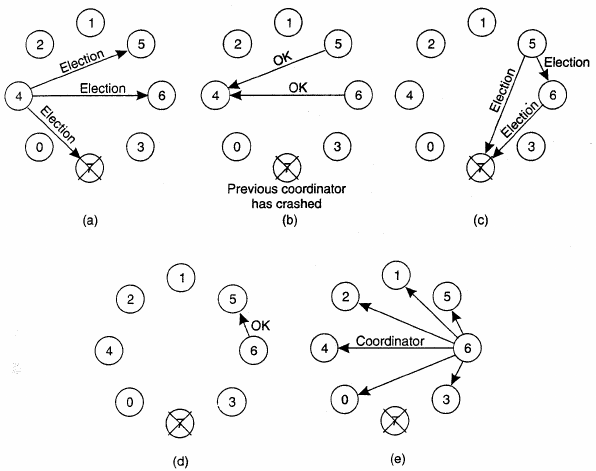
\includegraphics[width=0.7\linewidth]{bully_algorithm}
		\caption{Bully Algorithm}
		\label{fig:bullyalgorithm}
	\end{figure}
	
\end{frame}

% -----------------------------------------------------------------------------
\section{Preliminaries}
\subsection{System Model}

\begin{frame}{System Model}

\begin{itemize}
	\item We assume a system consisting of a set $P$ of computing nodes and a set $\chi$ of directed communication channels from one node to another node. $\chi$ consists of one channel.
	\item We model the whole system as a set of (infinite) state machines that interact through shared events (a specialization of the IOA model [17]).

\end{itemize}

\end{frame}


\subsection{Modeling Asynchronous Dynamic Links}
\begin{frame}{Asynchronous Dynamic Links' Model}

	The state of Channel(u, v), which models the communication channel from node u to node v, consists of:
	\begin{itemize}
		\item a $status_{uv}$ variable;
		\item and a queue $mqueue_{uv}$ of messages.
	\end{itemize}
	 

\end{frame}

\subsection{Configurations and Executions}
\begin{frame}

\end{frame}


\subsection{Problem Definition}

\begin{frame}{Heights}

The height for each node is a 7-tuple of integers $((\tau , oid, r), \delta, (nlts, lid), id)$, where the first three components are referred to as the reference level ($RL$) and the fifth and sixth.

\begin{itemize}
	\item $\tau$, a non-negative timestamp which is either 0 or the value of the causal clock time when the current search for an alternate path to the leader was initiated.
	\item $oid$, is a non-negative value that is either 0 or the id of the node that started the current search (we assume node ids are positive integers).
	\item $r$, a bit that is set to 0 when the current search is initiated and set to 1 when the current search hits a dead end.
	\item $\delta$

\end{itemize}

\end{frame}

% -----------------------------------------------------------------------------
\section{Leader Election Algorithm}
\subsection{Informal Description}
\begin{frame}{Heights}

The height for each node is a 7-tuple of integers $((\tau , oid, r), \delta, (nlts, lid), id)$, where the first three components are referred to as the reference level ($RL$) and the fifth and sixth.

\begin{itemize}
	\item $\tau$, a non-negative timestamp which is either 0 or the value of the causal clock time when the current search for an alternate path to the leader was initiated.
	\item $oid$, is a non-negative value that is either 0 or the id of the node that started the current search (we assume node ids are positive integers).
	\item $r$, a bit that is set to 0 when the current search is initiated and set to 1 when the current search hits a dead end.
	\item $\delta$

\end{itemize}

\end{frame}

\subsection{Nodes, Neighbors and Heights}
\begin{frame}{Heights}

The height for each node is a 7-tuple of integers $((\tau , oid, r), \delta, (nlts, lid), id)$, where the first three components are referred to as the reference level ($RL$) and the fifth and sixth.

\begin{itemize}
	\item $\tau$, a non-negative timestamp which is either 0 or the value of the causal clock time when the current search for an alternate path to the leader was initiated.
	\item $oid$, is a non-negative value that is either 0 or the id of the node that started the current search (we assume node ids are positive integers).
	\item $r$, a bit that is set to 0 when the current search is initiated and set to 1 when the current search hits a dead end.
	\item $\delta$

\end{itemize}

\end{frame}

\subsection{Initial State}
\begin{frame}{Heights}

The height for each node is a 7-tuple of integers $((\tau , oid, r), \delta, (nlts, lid), id)$, where the first three components are referred to as the reference level ($RL$) and the fifth and sixth.

\begin{itemize}
	\item $\tau$, a non-negative timestamp which is either 0 or the value of the causal clock time when the current search for an alternate path to the leader was initiated.
	\item $oid$, is a non-negative value that is either 0 or the id of the node that started the current search (we assume node ids are positive integers).
	\item $r$, a bit that is set to 0 when the current search is initiated and set to 1 when the current search hits a dead end.
	\item $\delta$


\end{itemize}

\end{frame}
\subsection{Goal Of The Algorithm}
\begin{frame}{Heights}

The height for each node is a 7-tuple of integers $((\tau , oid, r), \delta, (nlts, lid), id)$, where the first three components are referred to as the reference level ($RL$) and the fifth and sixth.

\begin{itemize}
	\item $\tau$, a non-negative timestamp which is either 0 or the value of the causal clock time when the current search for an alternate path to the leader was initiated.
	\item $oid$, is a non-negative value that is either 0 or the id of the node that started the current search (we assume node ids are positive integers).
	\item $r$, a bit that is set to 0 when the current search is initiated and set to 1 when the current search hits a dead end.
	\item $\delta$


\end{itemize}

\end{frame}
\subsection{Description Of The Algorithm}
\begin{frame}{Heights}

The height for each node is a 7-tuple of integers $((\tau , oid, r), \delta, (nlts, lid), id)$, where the first three components are referred to as the reference level ($RL$) and the fifth and sixth.

\begin{itemize}
	\item $\tau$, a non-negative timestamp which is either 0 or the value of the causal clock time when the current search for an alternate path to the leader was initiated.
	\item $oid$, is a non-negative value that is either 0 or the id of the node that started the current search (we assume node ids are positive integers).
	\item $r$, a bit that is set to 0 when the current search is initiated and set to 1 when the current search hits a dead end.
	\item $\delta$

\end{itemize}

\end{frame}


\subsection{Sample Execution}

\begin{frame}{The Code triggered by Update Message}
\begin{figure}[h]
	\centering
	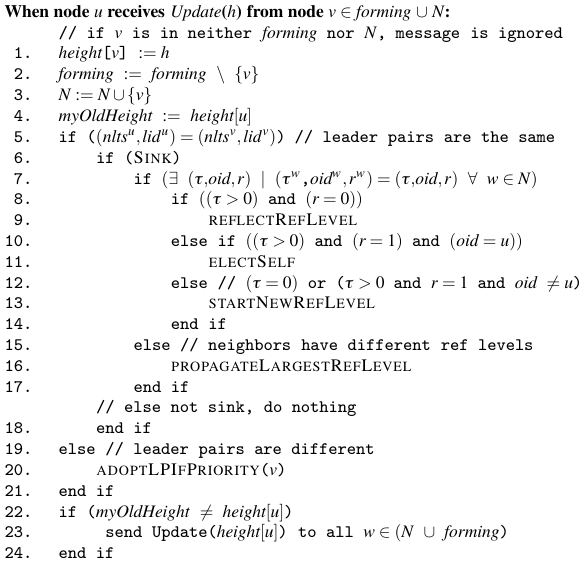
\includegraphics[width=0.6\linewidth]{tcode_update.png}
	%\caption{Code triggered by Update Message}
	\label{fig:figure1}
\end{figure}
\end{frame}

\begin{frame}{Subroutines}
\begin{figure}[h]
	\centering
	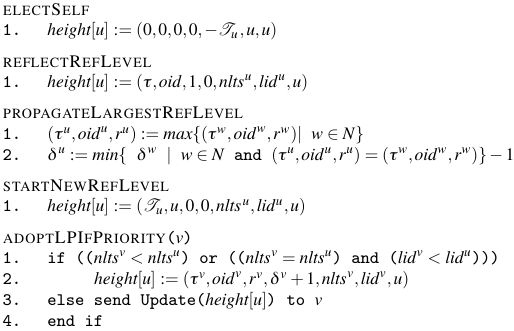
\includegraphics[width=0.8\linewidth]{subroutines.png}
	%\caption{Code triggered by Update Message}
	\label{fig:figure1}
\end{figure}
\end{frame}


% -----------------------------------------------------------------------------
\section{Correctness}

\subsection{Bounding the Number of Elections}

\subsection{Bounding the Number of New Reference Levels}

\subsection{Bounding the Number of Messages}
% -----------------------------------------------------------------------------

\section{Implementation}
\subsection{What's JBotSim ?}

\begin{frame}{What's JBotSim ?}

\end{frame}

%----------------------------------------------------------------------------
\section{Conclusions}
\subsection{Where can I learn more?}
\begin{frame}{Questions and Answers}
  Want to know more?

  \begin{itemize}
    \item Browse \url{http://web.mit.edu/smoot/history.htm}.
    \item Smoot's Legacy \url{http://alum.mit.edu/news/AlumniNews/Archive/smoots_legacy}.
    \item Smoot Salute! \url{http://web.mit.edu/spotlight/smoot-salute}.
  \end{itemize}
  
\end{frame}
% -----------------------------------------------------------------------------
\end{document}
